\documentclass[12pt]{article}
\usepackage[left=20mm, top=20mm, right=20mm, bottom=20mm, headsep=10pt]{geometry} 
\usepackage{cmap} % для кодировки шрифтов в pdf
\usepackage[T2A]{fontenc}
\usepackage[utf8]{inputenc}
\usepackage[russian]{babel}
\usepackage{graphicx} % для вставки картинок
\usepackage{amssymb,amsfonts,amsmath,amsthm,amsbsy} % математические дополнения от АМС
\usepackage{mathtools}
\usepackage{indentfirst} % отделять первую строку раздела абзацным отступом тоже
\usepackage{multicol}
%\usepackage{tempora}
\usepackage{epstopdf}
\usepackage{svg}
\usepackage{mathtools}
\usepackage{framed}
\usepackage{wrapfig}
\usepackage[font=small]{caption}
\usepackage{floatrow}
\floatsetup[table]{capposition=top}
\usepackage{subcaption}
\usepackage{titlesec}
\usepackage{setspace}
\usepackage{enumitem}
\usepackage{float}
\usepackage{epstopdf}
\usepackage{hepunits}
\usepackage[final]{pdfpages}
\usepackage{tikz}
\usepackage{authblk}
\usepackage{physics}

\usetikzlibrary{positioning,shapes,arrows}
%opening

\makeatletter
\renewcommand\AB@affilsepx{, \protect\Affilfont}
\makeatother

\title{Корректировка и настройка циркулярности поляризации лазерного поляриметра}
\author{Степан Захаров}
\begin{document}
\maketitle

\vspace{-3em} 
%\begin{abstract}
%\end{abstract}

\section{Постановка задачи}
Лазерный поляриметр ускорителя ВЭПП-4М базируется на принципе асимметрии обратного комптоновского рассеяния правых и левых циркулярно поляризованных фотонов на линейно поляризованных электронах. Степень поляризации электронов можно измерить, если зарегистрировать вертикальный сдвиг распределений обратно рассеянных квантов. Важно, что этот сдвиг линеен как по стоксовскому параметру $V$ лазерного пучка, так и по параметру поляризации электронного пучка $\mathcal{P}$:
\begin{equation}
\Delta y = \frac{\hbar \omega_0}{2 m_e c^2} \mathcal{P} \Delta V L,
\label{eq:pol_effect}
\end{equation}%
Для получения циркулярно поляризованных пучков используется следующая схема Рис. \ref{fig:LSRP_scheme}). Лазерное излучение генерируется неодимовым лазером и имеет на выходе из него линейную поляризацию. Проходя через фазовую пластинку, оси которой располагаются под углами $\pi/4$ к плоскости поляризации пучка лазера, пучок приобретает циркулярную поляризацию. Переключение между левой и правой циркулярностями происходит путем подачи высокого напряжения на ячейку Поккельса.
\begin{center}
	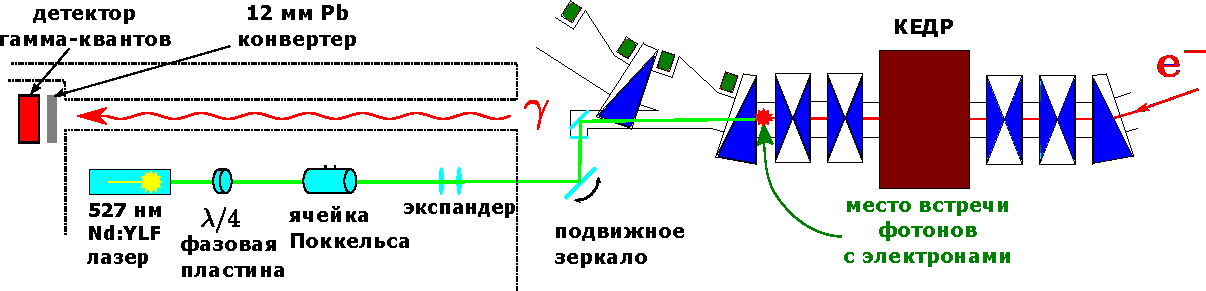
\includegraphics[width=16cm]{img/LSRP_scheme.pdf}
	\label{fig:LSRP_scheme}
\end{center}
Контроль циркулярности поляризации проводился с использованием специальной установки, которая состоит из вращающегося анализатора, установленного на шаговом двигателе, а также фотодетектора с поляризационным аттенюатором. Измеритель поляризации имеет возможность поворачивать анализатор на заданный угол т.е. определять не относительные поляризационные характеристики излучения,а абсолютные например в привязке к вертикальной оси).
\par Первичная настройка циркулярности проводилась на участке от ячейки Поккельса до экспандера. Нам удалось достичь значения циркулярности $V>0.99$. Для этого нужно сначала выставить оси фазовой пластинки, а затем, на включенной ячейке Поккельса добиться циркулярности поляризации.
\par Следующим этапом работы было измерение состояний поляризации после отражения от зеркал. Предыдущие эксперименты показали, что при отражении от одного зеркала циркулярность снижается примерно на $13\%$ По-видимому, это происходит из-за двух эффектов:
\begin{itemize}
	\item Различие коэффициентов отражения для TE и TM волн на зеркало летит суперпозиция двух волн с горизонтальной и вертикальной линейными поляризациями)
	\item Набег фаз между TE и TM волнами. 
\end{itemize}
Для того чтобы получить состояние поляризации, похожее на то, что образуется в вакуумной камере после отражения от двух зеркал одно из которых может ещё и иметь диэлектрическую пленку, было решено установить прямо у оптического ввода в камеру ещё одно зеркало и ориентировать его так же, как зеркало в камере. Далее по трассе пучка был расположен измеритель поляризации. Как оказалось, после двух отражений состояние поляризации сильно портится:
\begin{center}
	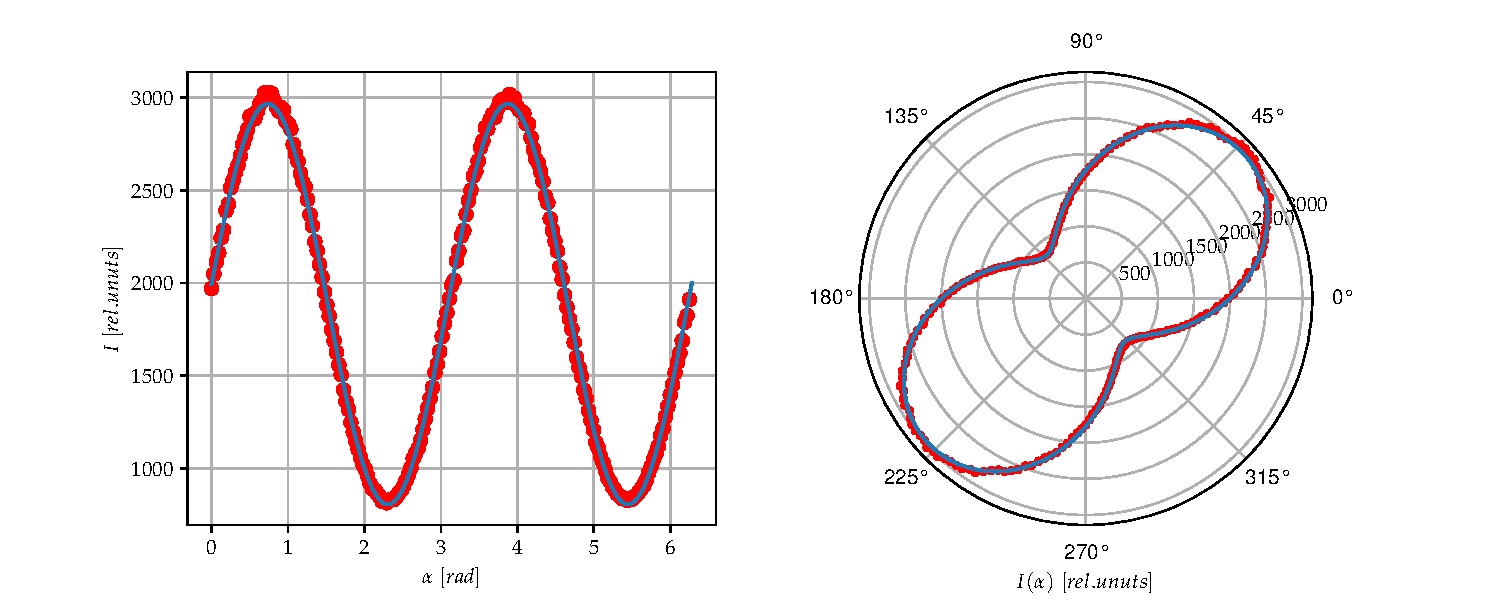
\includegraphics[width=16cm]{img/I_plot_no_corr}
	\label{fig:/I_plot_no_corr}
\end{center}

\begin{equation}
\vec{E} = \begin{bmatrix}{\hat{E_x}} \\ {\hat{E_y}} \end{bmatrix} = \begin{bmatrix*}[l]E_{x} \\ {E_y e^{i\psi}} \end{bmatrix*} = \begin{bmatrix*}[l] A \\ Be^{i\psi} \end{bmatrix*}
\tag{1}
\end{equation}
Измеритель поляризации чувствителен к интенсивности излучения т.е. к усредненному по времени значению электромагнитного поля.\par
Поляризатор, расположенный под углом $\alpha$ к горизонтали имеет следующую матрицу пропускания: 
\begin{equation}
\begin{split}
P(\alpha) &= \begin{pmatrix}\cos\alpha  &-\sin\alpha\\ \sin\alpha& \cos\alpha\\ \end{pmatrix}
 \begin{pmatrix}1&0\\0&0\end{pmatrix} \begin{pmatrix}\cos\alpha  &\sin\alpha\\ -\sin\alpha& \cos\alpha\\ \end{pmatrix}=  \begin{pmatrix}\cos^2\alpha &\cos\alpha \sin\alpha\\ \cos\alpha \sin\alpha& \sin^2\alpha\\ \end{pmatrix} \\ &= \frac{1}{2} \begin{pmatrix}\cos 2\alpha &\sin 2\alpha\\\sin 2\alpha& -\cos 2\alpha\\ \end{pmatrix} +\begin{pmatrix}1/2 & 0\\ 0& 1/2\\\end{pmatrix}
\end{split}
\end{equation}
При прохождении через поляризатор, вектор электромагнитного поля приобретет вид:
\begin{equation}
P(\alpha)\vec{E} =  \begin{bmatrix*}[l] A \cos^2 \alpha + Be^{i\psi} \cos\alpha \sin \alpha \\A \cos\alpha \sin \alpha + Be^{i\psi} \sin^2 \alpha  \end{bmatrix*}
	\tag{1}
	\end{equation}

\begin{equation}
\begin{split}
I &= \langle E^2 \rangle_t  = \bigg \langle \begin{bmatrix}\hat{E_x} & \hat{E_y}\\ \end{bmatrix}^* \begin{bmatrix}\hat{E_x}\\ \hat{E_y} \end{bmatrix} \bigg\rangle_t =  \langle E_x^2 \rangle_t + \langle E_y^2 \rangle_t =\\ &A^2 \cos^4 \alpha + B^2 \cos^2 \alpha \sin^2 \alpha + AB \cos \psi \cos^3 \alpha \sin \alpha~+ \\ &B^2 \sin^4 \alpha + A^2 \cos^2 \alpha \sin^2 \alpha + AB \cos \psi  \cos \alpha \sin^3 \alpha = \\
   & A^2 \cos^2 \alpha + B^2 \sin^2 \alpha + AB \cos \psi \sin 2 \alpha.  
\end{split}
\label{I2angle}
\end{equation}

Удобно преобразовать полученное выражение \ref{I2angle} так, чтобы выделить осциллирующую и постоянную части:
\begin{equation}
A^2 \cos^2 \alpha + B^2 \sin^2 \alpha + AB \cos \psi \sin 2 \alpha = \frac{A^2 + B^2}{2} + \bigg[\frac{A^2 - B^2}{2} \cos 2\alpha + AB \cos \psi \sin 2 \alpha \bigg] \\\label{I2transformed1}
\end{equation}
\begin{equation}
= \frac{A^2 + B^2}{2} + C\cdot\big[\sin 2\beta \cos 2\alpha + \cos 2\beta \sin 2 \alpha\big] = \frac{A^2 + B^2}{2} + C\cdot \sin (2 [\beta + \alpha])
\label{I2transformed2}
\end{equation}
Здесь угол $\beta$ - дополнительный угол к тому, что показывает поворот главных осей эллипса относительно лабораторных осей, а коэффициент $C$ является амплитудой колебаний графика интенсивности:
\begin{align}
	\beta = \frac{1}{2}\atan\bigg(\frac{A^2 - B^2}{2AB\cos \psi}\bigg) \\
	 C = \sqrt{\bigg[\frac{A^2 - B^2}{2}\bigg]^2 + [AB \cos \psi]^2}
\end{align}
\textbf{$\mathrm{N}\!\!\mathrm{B}$:} объясним дополнительно момент с углами на примере. Если сдвиг фаз $\psi =0$, то этому соответствует линейная поляризация с плоскостью, расположенной под углом $\pi/4$ к главным осям. Распределение интенсивности имеет следующий вид: 
\begin{center}
	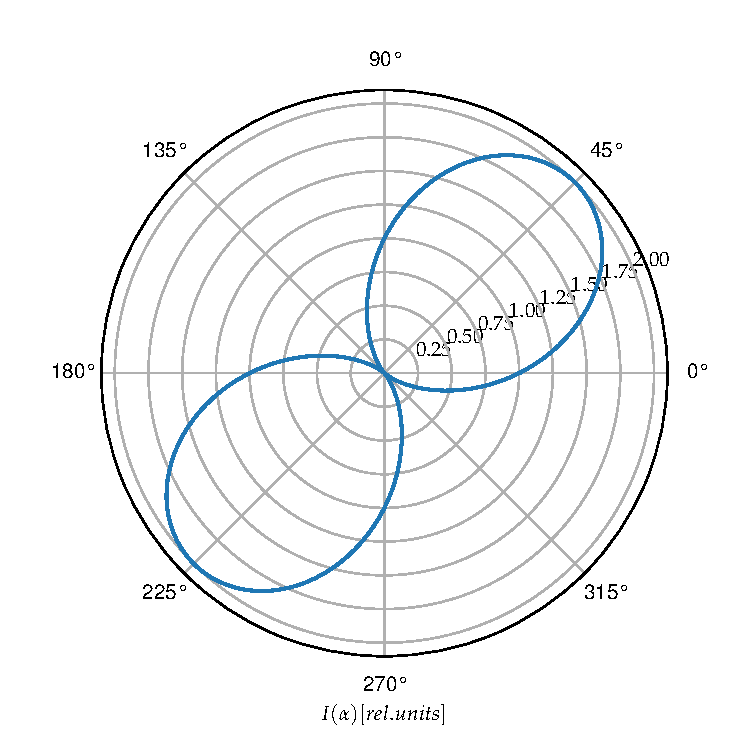
\includegraphics[width=8cm]{img/linpol_polar}
	\label{fig:/linpol_polar}
\end{center}
С другой стороны, колебания интенсивности описываются формулой \ref{I2transformed2}, в которой колебательный член $\sim \sin(2 [\beta + \alpha])$, и максимум для такого случая наблюдается при $2[\beta+\alpha]=\pi/2$.  Чтобы получить распределение интенсивности как на Рис. \ref{fig:/linpol_polar}, угол $\beta$ должен равняться нулю, а $\alpha$, соответственно равняется $\pi/4$ . Таким образом можно интерпретировать угол $2\beta$ как дополнительный к удвоенному углу наклона главных осей эллипса поляризации.
 
После выделения в формуле \ref{I2transformed2} осциллирующей части, становится понятно, что причин колебаний значения интенсивности при повороте поляризатора две:
\begin{itemize}
	\item  $A \neq B =>$ при отражении от зеркал различаются коэффициенты отражения для TE и TM волн
	\item После отражения от зеркал между вертикальной и горизонтальной компонентой набегает дополнительный сдвиг фаз
\end{itemize}
Поймем, какой эффект является превалирующим? Для аппроксимируем график интенсивности функцией \ref{I2transformed1}.
Параметры, полученные из фита: 
\begin{center}
	\begin{tabular}{|c|c|c|} 
		\hline
		Параметр & Значение & Ед. изм.\\
		\hline
		$A^2$ & $1994.5\pm0.2$ & бин АЦП \\ 
		\hline
	 	$B^2$ & $1778. 4\pm0.2$ & бин АЦП \\ 
		\hline
		$\psi$ & $55.2\pm0.1$ & град. \\
		\hline
	\end{tabular}
\end{center}
Сравнивать нужно коэффициенты перед синусом и косинусом $2\alpha$:
\begin{align}
	\frac{A^2 - B^2}{2} = 108.1\pm 0.4 \quad AB \cos \psi = 1079\pm 2 
	\label{errors}	
\end{align}
Эффект разницы осей на порядок меньше, чем осцилляции интенсивности из-за сдвига фазы. Необходимо компенсировать $35^{\circ}$, чтобы достичь примерно $10\%$ примеси линейной поляризации. \par
После оценок решено было установить корректирующую ячейку Поккельса и ориентировать её по главным осям системы. Делать это лучше всего на циркулярной поляризации и особую тщательность проявлять при настройке оптических осей. В курсовой работе 2017 года мной проводилось измерение полуволнового напряжения на данной ячейке, что помогло оценить примерное напряжение в районе 500-800В. 
\begin{center}
	\begin{figure}[H]
		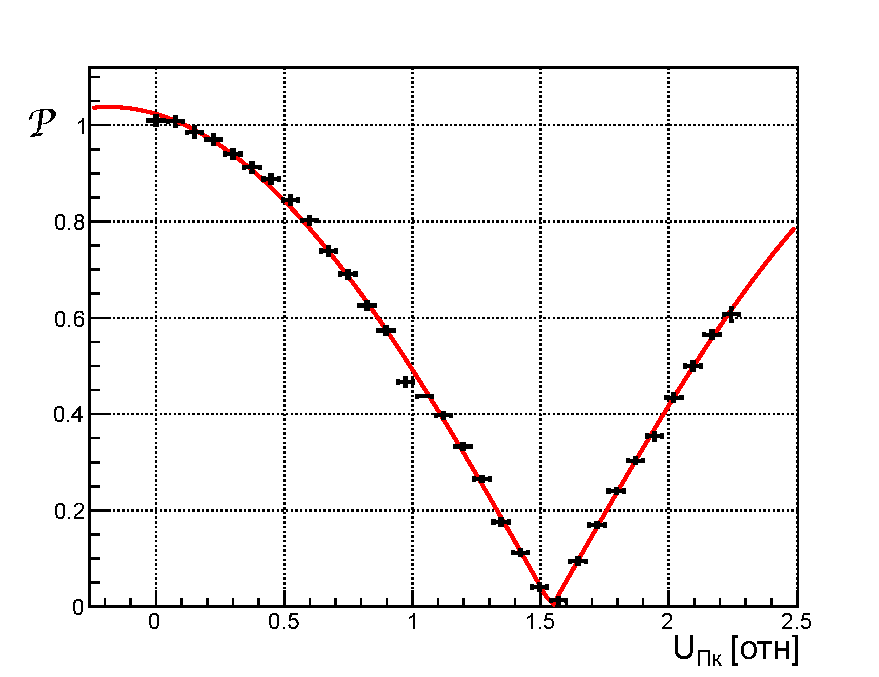
\includegraphics[width=8cm]{img/dphi2U_Pokkels.pdf}
		\label{fig:dphi2U_Pokkels}
		\caption{Зависимость параметра поляризации $\mathcal{P}\sim |\cos \delta \psi|^2$ от полуволнового напряжения. Сдвиг фаз $\delta \psi$ линеен по полю => по напряжению питания. По горизонтальной оси напряжение в В}
	\end{figure}
\end{center}
Значение напряжения, при котором был достигнут наилучший эффект -- 800В, что соответствует сдвигу фазы порядка $40^{\circ}$ и находится в согласии с предсказанием расчетов. 
График интенсивности после корректировки имеет следующий вид: 
\begin{center}
	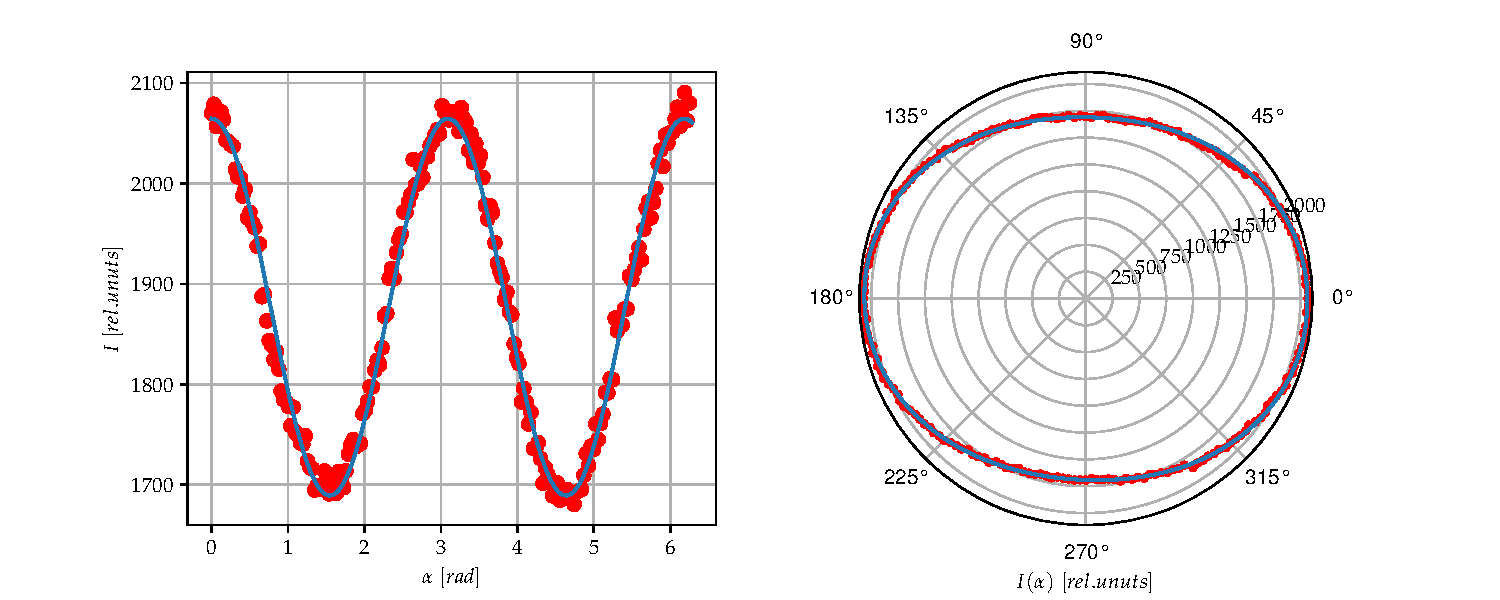
\includegraphics[width=16cm]{img/I_plot_corr}
	\label{fig:/I_plot_corr}
\end{center}
Параметры, полученные из фита: 
\begin{center}
	\begin{tabular}{|c|c|c|} 
		\hline
		Параметр & Значение & Ед. изм.\\
		\hline
		$A^2$ & $2064.6\pm0.1$ & бин АЦП \\ 
		\hline
		$B^2$ & $1689.2\pm0.1$ & бин АЦП \\ 
		\hline
		$\psi$ & $90.00\pm0.07$ & град. \\
		\hline
	\end{tabular}
\end{center}
Отношение осей эллипса поляризации составляет $9.5\%$ и соответствует значению параметра стокса $Q=0.1$. Требуется дальнейшая настройка, однако уже получено улучшение в 6 раз (до калибровки примесь линейной оценивалась как $U=0.6$ т.к. эллипс был ориентирован под углом почти $45^{\circ}$ к главным осям).\par
Дальнейшее улучшение заключается в повороте осей корректирующей ячейки Поккельса, чтобы приготовить состояние поляризации не только со сдвинутыми фазами, но ещё и с разными амплитудами по главным осям.  


\vfill
\end{document}
